\chapter{Una introducción a NuSA}

\section{¿Qué es NuSA?}

\textbf{NuSA} es una librería Python para resolver problemas de análisis estructural bidimensional. 
La idea es tener una estructura de códigos escritos utilizando la programación orientada a 
objetos, de modo que sea posible crear instancias de un modelo de elemento finito y operar 
con éste mediante métodos de clase.\\

La estructura de \textbf{NuSA} está basada en tres clases fundamentales que componen el \textit{core}: 
\texttt{Model}, \texttt{Node} y \texttt{Element}.

\begin{center}
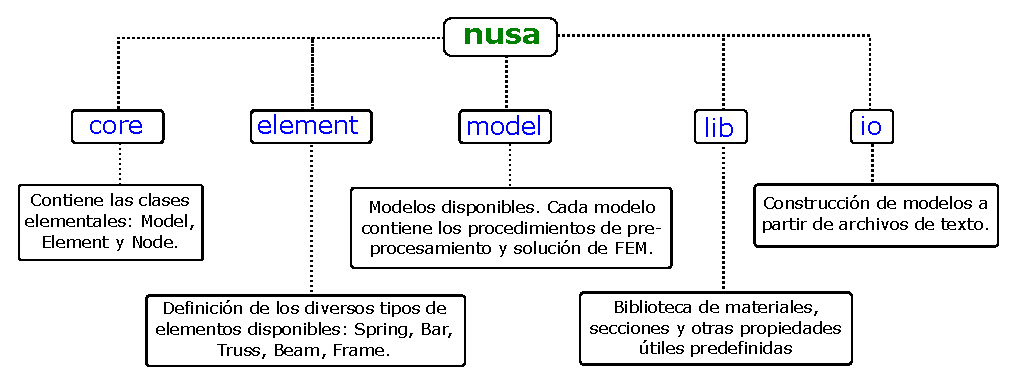
\includegraphics[scale=0.8]{src/intro-nusa/nusa_structure.eps}
\end{center}


\begin{python}
class Model(object):
    """
    Superclass for all FEA models
    """
    def __init__(self,name,mtype):
        self.mtype = mtype # Model type
        self.name = name # Name 
        self.nodes = {} # Dictionary for nodes {number: NodeObject}
        self.elements = {} # Dictionary for elements {number: ElementObject}
        
    def addNode(self,node):
        """
        Add element to current model
        
        *node* :   :class:`~nusa.core.Node`
        """
        current_label = self.getNumberOfNodes()
        if node.label is "":
            node.setLabel(current_label)
        self.nodes[node.label] = node
        
    def addElement(self,element):
        """
        Add element to current model
        
        *element* :  :class:`~nusa.core.Element`
            Element instance 
        
        ::
        
            m1 = Model()
            e1 = Bar(Node((0,0),0),Node((1,0),0))
            m1.addElement(e1)
        
        """
        if self.mtype != element.etype:
            raise ValueError("Element type must be "+self.mtype)
        current_label = self.getNumberOfElements()
        if element.label is "":
            element.setLabel(current_label)
        self.elements[element.label] = element

    def getNumberOfNodes(self):
        return len(self.nodes)
        
    def getNumberOfElements(self):
        return len(self.elements)
        
    def getNodes(self):
        return self.nodes.values()
        
    def getElements(self):
        return self.elements.values()
    
    def __str__(self):
        custom_str = ("Model: "+self.name+"\nNodes: "+str(self.getNumberOfNodes())+
        "\nElements: "+str(self.getNumberOfElements()))
        return custom_str
\end{python}